
\chapter{Introducción. ¿Qué es un SIG?}
\label{Introduccion_fundamentos}



\bigskip

\begin{intro}
Este capítulo presenta los conceptos fundamentales sobre Sistemas de Información Geográfica (SIG), definiéndolos y presentando tanto sus capacidades fundamentales como la forma en que estas pueden ser aprovechadas. Asimismo, se presentan los SIG como sistemas complejos, y se describe cada uno de sus componentes principales. El capítulo presenta una visión global del ámbito de los SIG y de la ciencia asociada a los SIG como disciplina independiente, al tiempo que muestra el contexto en el que el desarrollo y utilización de estos se produce en la actualidad.
\end{intro}

\section{Introducción}
\pagestyle{fancy}

La mayor parte de la de la información que manejamos en cualquier tipo de disciplina está georreferenciada. Es decir, que se trata de información a la cual puede asignarse una posición geográfica, y es por tanto información que viene acompañada de otra información adicional relativa a su localización. 

Si bien esto no es un hecho novedoso, la situación actual es más favorable que nunca para el desarrollo de herramientas que permitan la utilización de toda esa información al tiempo que se consideran los datos relativos a su posición en el espacio. Esto es así no solo porque trabajamos con gran cantidad de información referenciada geográficamente, sino porque somos cada día más conscientes de la importancia que esa componente geográfica tiene. La geografía ha pasado de ser un ámbito particular con cierta relación con otros campos a ser un elemento fundamental incorporado a la mayor parte de las disciplinas. Y no solo en el terreno científico, sino en el terreno mismo de la vida diaria, donde toda esta información desempeña un papel de gran importancia.

La utilización de cartografía ha dado un vuelco radical en el plazo de unas décadas, permitiendo nuevas posibilidades y acercando la información cartográfica como herramienta de primer orden a un público amplio y diverso. La elaboración misma de cartografía ha pasado de ser terreno exclusivo de profesionales del sector a ser una labor abierta donde las nuevas tecnologías, especialmente las de corte colaborativo, han permitido que otro tipo de usuarios desarrollen y compartan información cartográfica.

En este sentido, los SIG no son solo herramientas dentro de ese contexto de gran importancia de la información geográfica, sino en gran medida responsables de que esa situación sea tal, pues su contribución dentro del panorama relativo a la geografía ha sido vital para impulsar esta y hacerla llegar hasta su lugar actual. En una sociedad donde la información y la tecnología son dos de los pilares fundamentales, los SIG son, sin lugar a dudas, la tecnología estandarte para el manejo de información geográfica, y los elementos básicos que canalizan la gestión de todo aquello que, de un modo u otro, presente una componente geográfica susceptible de ser aprovechada.

Así, un SIG es fundamentalmente una herramienta para trabajar con información georreferenciada, una definición en la que pueden entrar un gran número de tecnologías y de otros elementos no tecnológicos, los cuales veremos a lo largo de este libro.


\section{Un pequeño ejemplo}

Para comenzar a tener una idea correcta de lo que representa e implica un SIG, veamos un sencillo ejemplo. Supongamos el caso de un organismo o empresa cuyo trabajo incluye la gestión de una masa forestal. Este trabajo de gestión implicará algunas actividades como las siguientes, en las cuales se utiliza en mayor o menor medida información georreferenciada.

\begin{itemize}
	\item Delimitación de las distintas zonas inventariables y unidades dasocráticas (montes, cantones, rodales, etc.)
	\item Diseño de inventarios
	\item Realización de inventarios y gestión de sus datos para la obtención de resultados tales como estimaciones de volúmenes maderables.
	\item Gestión de infraestructuras del monte tales como vías de comunicación, torres de vigilancia contra incendios, etc.
\end{itemize}

En un contexto en el que no existen medios informáticos para la realización de estas tareas, gran parte de ellas se desarrollarán con el apoyo de cartografía clásica. Así, las zonas inventariables se delimitarán sobre un plano, y sobre este mismo pueden medirse sus superficies con la ayuda de un planímetro. En ese mismo plano se localizan las parcelas a muestrear en un inventario, y los operarios encargados de llegar hasta esas parcelas y realizar las mediciones pertinentes se ayudan de él para localizarlas y desplazarse sobre el terreno.

Los resultados del inventario se almacenan en estadillos, y las operaciones correspondientes al análisis estadístico de estos se realizan de forma manual, así como la comparación con inventarios anteriores que permiten estudiar la evolución del monte.

La presencia de medios informáticos facilita estas tareas, mejorando por una parte la gestión de los datos, y por otra las operaciones que pueden realizarse sobre estos. Una sencilla hoja de cálculo, por ejemplo, es una herramienta imprescindible para la gestión de los datos de un inventario, haciendo que todo el trabajo con ellos resulte más eficiente y adecuado.

En lo relativo a la cartografía, la situación, aunque con un desarrollo (y especialmente una implantación de usuarios) más reciente, no es muy distinta. Ventajas similares a las que aporta una hoja de cálculo pueden encontrarse en una aplicación que permitiera utilizar mapas y planos \emph{dentro} de un ordenador, con la consecuente ganancia en productividad, eficiencia y precisión. Esta aplicación destinada al manejo de cartografía es el concepto básico de un Sistema de Información Geográfica, y la idea fundamental a partir de la cual comenzó el desarrollo de estos.

Con un SIG, la cartografía de esa masa forestal puede visualizarse y almacenarse en un ordenador personal, y pueden realizarse sin dificultad y de forma instantánea cálculos tales como mediciones de cada una de las entidades. La creación de nueva información cartográfica se lleva a cabo ya en el propio SIG, del mismo modo que la edición de cartografía ya existente. Modificar el límite de una unidad dasocrática o el trazado de una vía, o crear la cartografía correspondiente a las parcelas de inventario son tareas que, en nuestro caso de ejemplo, se realizan hoy en día empleando un SIG.

Las ventajas que esto tiene son muchas, especialmente las relacionadas con una mejor gestión del conjunto de distintos datos que se manejan, así como las relativas a la sencillez con que pueden modificarse estos datos\footnote{Veremos con más detalle las ventajas de los datos digitales frente a los datos analógicos en el capítulo \ref{Fuentes_datos}}.

Otras de las labores donde un SIG demuestra su utilidad es en el análisis. Los datos geográficos pueden ser objeto de gran número de distintos análisis, y la capacidad de cómputo de un ordenador es necesaria para muchos de ellos. La herramienta idónea para implementar esos algoritmos y operaciones de análisis espacial es el SIG, pues ya contiene los elementos necesarios para el manejo de los datos de partida, es decir, aquellos que contienen la información georreferenciada.

Y, por supuesto, un SIG conectado a un periférico de impresión permite generar una versión analógica a partir de la información con la que se trabaja, teniendo la capacidad de crear cartografía en papel cuando así se requiera.

En otras palabras, un SIG es una herramienta que brinda a las labores de uso y manejo de información geográfica toda la potencia de un ordenador, pues ha sido diseñada específicamente para trabajar con este tipo particular de información.

No obstante, más allá de todas estas tareas antes mencionadas el concepto de SIG ha evolucionado hasta convertir actualmente a estos en sistemas complejos que buscan dar solución a todas las necesidades que se presentan en situaciones similares a la del ejemplo comentado. Con la tecnología actual, la incorporación de elementos propios de los SIG puede llegar mucho más allá, y uno de los pilares más sólidos de los SIG en la actualidad es su capacidad de mostrar que existe una componente espacial susceptible de ser gestionada con la ayuda de un SIG en la práctica totalidad de contextos posibles.

Como sistema, un SIG puede gestionar la cartografía necesaria para la gestión integral del monte, y hacerlo además de forma centralizada. De este modo, se garantiza el rigor y la robustez de los datos base, ya que el SIG es el encargado de canalizar la utilización de estos por parte de todos los usuarios. Esto es de especial importancia en caso de que se editen los datos, ya que esta edición también está centralizada, y un usuario ve reflejarse en su cartografía de forma inmediata los cambios realizados por otro, teniendo siempre a su disposición la versión más actual y, por tanto, más adecuada.
 
A esto puede añadirse la utilización de SIG móviles en dispositivos portátiles, que permiten que el SIG se incorpore también a las fases de trabajo de campo. Esa misma cartografía centralizada pueden utilizarla los operarios en campo a través de sus dispositivos para desarrollar su trabajo, ayudándose además de sistemas de navegación para la localización de las parcelas de un muestreo o de cualquier otro punto de interés al que deban desplazarse. 

Gracias a la tecnología SIG, la información espacial puede ser aprovechada en mayor medida, y en muchos casos pasa de ser una información inherente a los datos pero sin una verdadera aplicación, a ser un elemento sumamente enriquecedor y clave para muchos análisis. 

En nuestro ejemplo de gestión forestal, los propios datos del inventario, que antes eran fundamentalmente datos sobre las propiedades de los distintos árboles medidos (altura, diámetro, etc.), ahora ofrecen muchas más posibilidades si se considera que cada uno de estos árboles ha sido medido en una parcela dada, la cual lleva asociadas unas coordenadas concretas.

El trabajo que se desarrollaba en la hoja de cálculo con estos datos se puede incorporar al SIG, el cual además de las funciones de análisis estadístico incluye funciones de análisis espacial. De este modo, los resultados numéricos que se obtenían de esos análisis (volúmenes totales estimados, alturas medias, etc.) se amplían mediante resultados con mayor componente espacial, como puede ser la creación de nueva cartografía referente a las variables principales (mapas de densidad media de arbolado, altura dominante media, etc.). 

En resumen, el SIG en su concepción actual es una herramienta integradora que busca abarcar en su ámbito todas las funcionalidades que se requieren para el trabajo con variables y elementos espacialmente localizados, incorporando para ello capacidades variadas que serán las que vayamos viendo progresivamente a lo largo de esta obra.

\section{¿Qué es un SIG?}

Partiendo del ejemplo anterior, podemos dar una definición más precisa y formal de lo que realmente es un SIG. Básicamente, un SIG ha de permitir la realización las siguientes operaciones:

\begin{itemize}
	\item Lectura, edición, almacenamiento y, en términos generales, gestión de datos espaciales.
	\item Análisis de dichos datos. Esto puede incluir desde consultas sencillas a la elaboración de complejos modelos, y puede llevarse a cabo tanto sobre la componente espacial de los datos (la localización de cada valor o elemento) como sobre la componente temática (el valor o el elemento en sí).
	\item Generación de resultados tales como mapas, informes, gráficos, etc.
\end{itemize}

En función de cual de estos aspectos se valore como más importante, encontramos distintas definiciones formales del concepto de un SIG. Una definición clásica es la de \cite{Tomlin1990Prentice}, para quien un SIG es un elemento que permite <<analizar, presentar e interpretar hechos relativos a la superficie terrestre>>. El mismo autor argumenta, no obstante, que <<esta es una definición muy amplia, y habitualmente se emplea otra más concreta. En palabras habituales, un SIG es un conjunto de \emph{software} y \emph{hardware} diseñado específicamente para la adquisición, mantenimiento y uso de datos cartográficos>>.

En una línea similar, \cite{Star1990Prentice} define un SIG como un <<sistema de información diseñado para trabajar con datos referenciados mediante coordenadas espaciales o geográficas. En otras palabras, un SIG es tanto un sistema de base de datos con capacidades específicas para datos georreferenciados, como un conjunto de operaciones para trabajar con esos datos. En cierto modo, un SIG es un mapa de orden superior>>.

Ambas definiciones recogen el concepto fundamental de los SIG en el momento en que fueron escritas, pero la realidad hoy en día hace necesario recoger otras ideas, y la definición actual de un SIG debe fundamentarse sobre todo en el concepto de \emph{sistema} como elemento integrador que engloba a un conjunto de componentes interrelacionados.

Como apunta \cite{Tomlin1990Prentice}, \emph{software} y \emph{hardware} son dos elementos primordiales del SIG, pero no son sin embargo los únicos. En el contexto actual, otros componentes juegan un papel igual de importante en la idea global de un SIG.

De igual modo, un SIG puede considerarse como un <<mapa de orden superior>> entendiendo que se trata de una forma más potente y avanzada de hacer todo aquello que, previamente a la aparición de los SIG, se llevaba a cabo mediante el uso de mapas y cartografía en sentido clásico. Es decir, los SIG representan un paso más allá de los mapas. No obstante, esta definición resulta en exceso simplista, pues mapas y SIG no son conceptos equiparables en el contexto actual de estos últimos. 

Un mapa es una representación de un conjunto de datos espaciales y, aunque esta representación resulta de enorme importancia, en el entorno de un SIG no es sino un elemento más de una serie de componentes (tales como el \emph{software} y el \emph{hardware} que antes mencionábamos). Más aún, un SIG contiene no solo los datos y la representación, sino también las operaciones que pueden hacerse sobre el mapa, que no son ajenas a este sino partes igualmente de todo el sistema conformado por el SIG.

De la misma forma que los textos han pasado del papel al ordenador (antes leíamos libros, ahora podemos leer libros impresos, libros digitales, páginas Web, etc.), los mapas también han dado ese salto cualitativo con la aparición de los SIG. Sin embargo, el SIG es mucho más que una nueva forma de cartografía, y no invalida en absoluto formas anteriores. De hecho, una función muy importante de los SIG es ayudar a crear mapas en papel, y estos se siguen utilizando hoy en día en todos los ámbitos. Y junto con esta funcionalidad, encontramos otras que hacen que en su conjunto un SIG sea una herramienta integradora y completa para el trabajo con información georreferenciada.

Debe entenderse, pues, un SIG, como un elemento complejo que engloba una serie de otros elementos conectados, cada uno de los cuales desempeña una función particular. Estos elementos son, como iremos viendo más adelante, los datos, los procesos, la visualización, la tecnología y el factor organizativo. Baste por el momento citarlos, ya que más adelante, y a lo largo de todo el libro, se irán describiendo pormenorizadamente todos ellos.

Con lo anterior, una definición más precisa es decir que un SIG es un sistema que integra tecnología informática, personas e información geográfica\cite{webGISCOM}, y cuya principal función es capturar, analizar, almacenar, editar y representar datos georreferenciados \cite{Korte2001Autodesk}.

En las siguientes secciones veremos por separado la forma en que un SIG integra la tecnología informática, las personas y la información geográfica, así como la forma en que los conceptos fundamentales en los que el propio SIG se sustenta suponen una integración de distintas disciplinas.

\subsection{SIG como integrador de información}

Si bien un SIG tiene una inherente naturaleza integradora y esta puede enfocarse desde muchos puntos de vista tal y como vemos en este apartado, el elemento tal vez más relevante en este sentido es la propia información que un SIG maneja y las características de esta. Conceptualmente, el verdadero pilar de esa naturaleza integradora del SIG reside en la información geográfica con la que se trabaja, que provee la amalgama adecuada para que un SIG sea un sistema sólido y cohesionado, confiriéndole a su vez sus propias características y su interés como herramienta polivalente.

Muchas disciplinas trabajan con información de distinta naturaleza. En ellas, no siempre resulta sencillo buscar elementos en común para poder unir y coordinar toda esa información bajo un único punto de vista conceptual. En otras ocasiones, disciplinas que en la práctica presentan una interacción real (puede decirse que, de un modo u otro, todas las disciplinas están interrelacionadas) resultan difíciles de integrar desde el punto de vista teórico, y no es sencillo ponerlas en un marco común de trabajo.

Por ejemplo, información de tipo sociológico como la tasa de analfabetismo e información de carácter físico o biológico como puede ser la acidez del suelo, no parecen sencillas de combinar para la realización de algún análisis común. De existir alguna relación entre ellas (o de no existir, y pretender demostrar que son variables independientes), es necesario buscar un punto de enlace entre ambas informaciones para poder estudiar esta. Un nexo que las une es el hecho de que están asociadas a una localización en el espacio, ya que una serie de datos de tasa de analfabetismo corresponderán a una serie de lugares, del mismo modo que lo harán los valores de acidez del suelo. 

El hecho de que ambas informaciones tienen a su vez carácter geográfico va a permitir combinarlas y obtener resultados a partir de un análisis común. Puesto que, tal y como se mencionó al inicio de este capítulo, aproximadamente un 70\% de toda la información está georreferenciada, esa georreferencia va a representar en una gran mayoría de los casos un punto común para enmarcar el análisis. El SIG es, en este contexto, el marco necesario en el que incorporar esa información georreferenciada y trabajar con ella.

\subsection{SIG como integrador de tecnologías}

Puede pensarse que los SIG son meramente herramientas informáticas y que la única tecnología que reside tras ellas es la propia tecnología informática. Sin embargo, el papel integrador de los SIG hace que sean la herramienta elegida para la gestión de resultados y elementos producidos por otras tecnologías, muchas de las cuales se encuentran actualmente en pleno desarrollo. 

La popularización de los SIG y su mayor presencia en una buena parte de los ámbitos de trabajo actuales han traído como consecuencia una mayor  conciencia acerca de la importancia de la componente espacial de la información, así como sobre las posibilidades que la utilización de esta ofrece. Por ello, una gran parte de las tecnologías que han surgido en los últimos años (y seguramente de las que surjan en los próximos) se centran en el aprovechamiento de la información espacial, y están conectadas en mayor o menor medida a un SIG para ampliar su alcance y sus capacidades. Por su posición central en el conjunto de todas las tecnologías, los SIG cumplen además un papel de unión entre ellas, conectándolas y permitiendo una relación fluida alrededor de las funcionalidades y elementos base de un Sistema de Información Geográfica.

\subsection{SIG como integrador de personas}

Ya sabemos que la información georrefenciada es muy numerosa y variada. Esto significa que son muchos los tipos de personas que pueden emplearla y, por tanto, que pueden emplear un SIG para el trabajo con ella. La presencia del SIG como puerta de acceso a esa información es un punto común a todas esas distintas personas, y un Sistema de Información Geográfica es también un elemento integrador a nivel humano y profesional.

Dentro incluso de un mismo campo de aplicación, son varios los grupos de personas que van a estar implicados en el desarrollo de una tarea dada con la ayuda de un SIG. Desde la creación del dato geográfico hasta la obtención de un resultado final son muchas las operaciones que se llevan a cabo, y estas las desarrollan profesionales de distinta especialización y con herramientas particularmente adaptadas a dichas operaciones. En nuestro ejemplo, y en la etapa previa a la aparición de los SIG, las herramientas que emplea el cartógrafo para generar un mapa son muy diferentes de las que emplea el gestor para analizar dicho mapa, y estas a su vez distintas a las que pueden emplearse para la elaboración de resultados. 

Con la aparición de los SIG, todos los profesionales dentro de esa cadena que va desde la creación del dato hasta las operaciones finales que se realizan sobre estos tienen una herramienta común de trabajo, pues un SIG puede utilizarse para desarrollar parcial o totalmente las tareas correspondientes a cada uno de ellos. El SIG es empleado para crear cartografía, para almacenar, gestionar y consultar esta, así como para realizar análisis más complejos en base a ella y crear resultados.

Las funciones básicas que un SIG ha de cumplir, que ya vimos en el momento de dar una definición de estos, cubren en realidad un rango amplio de trabajo, y engloban las necesidades de usuarios que con anterioridad no tenían entre sí un marco de trabajo común tan definido. Esto tiene como consecuencia que existe una mejor coordinación entre ellos, pues es la propia herramienta quien establece las características de la relaciones existentes, y estas no dependen ya únicamente del propio ámbito de aplicación. No obstante, aparece una mayor necesidad de organización, y como veremos más adelante, esta organización es una de las partes básicas del sistema SIG y un elemento necesario para su buen funcionamiento.

\subsection[SIG como integrador de teorías y fundamentos]{SIG como integrador de teorías y fundamentos. La Ciencia de la Información Geográfica}

La evolución conceptual que se ha producido en el ámbito de los SIG, pasando como ya hemos visto de ser considerados simples programas informáticos a sistemas completos con múltiples componentes, ha tenido lugar también en la ciencia que los rodea. Los SIG no solo han contribuido al desarrollo de las ciencias afines, sino que en muchos casos han modificado estas o han contribuido a la formación de nuevas ramas. Conceptos básicos y hasta ese momento sólidos,  como por ejemplo la idea de lo que es y lo que significa un mapa (una idea fundamental para el trabajo en muchas disciplinas), han sido literalmente redefinidas desde la aparición de los SIG.

Desde un punto de vista muy simple, podemos entender un SIG como la unión de dos ciencias: la geografía y la informática. Visto así, un SIG es una herramienta informática para ayudar al trabajo en el ámbito geográfico. Esta concepción tan simple dista, no obstante, mucho del concepto real de un SIG, pues este incorpora elementos de muchas ciencias distintas como pueden ser las siguientes\cite{webGoodchildNCGIA}:

\begin{itemize}
	\item Disciplinas relacionadas con la tecnología y el manejo de información. Se incluyen aquí las ciencias de la información, la informática, el diseño de bases de datos o el tratamiento digital de imágenes, entre otras. Muchas de estas, a su vez, derivan de otras o toman importantes elementos de ellas. La estadística o la matemática son algunas de esas ciencias fundamentales.
	\item Disciplinas dedicadas al estudio de la Tierra desde un punto de vista físico. La geología, la oceanografía, la ecología, así como todo el conjunto de ciencias medioambientales, forman parte de este grupo.
	\item Disciplinas dedicadas al estudio de la Tierra desde un punto de vista social y humano. En este grupo se incluyen la antropología, la geografía o la sociología, entre otras. Las ciencias de este grupo, así como las del anterior, son todas ellas potenciales usuarias de los SIG.
	\item Disciplinas dedicadas al estudio del entendimiento humano, en particular en lo concerniente a la interacción con máquinas. Las ciencias del conocimiento, la psicología en general o las ramas que estudian y desarrollan la Inteligencia Artificial también juegan su papel en el contexto actual de los SIG.
	\item Disciplinas que tradicionalmente han realizado una integración de conocimientos de otros ámbitos distintos. La geografía como tal es la principal representante de este grupo.
\end{itemize}

En el contexto presente, podemos entender la Ciencia de la Información Geográfica\footnote{\emph{Geographic Information Science} en inglés, abreviado como GIScience o simplemente con el propio acrónimo GIS} como todo el conjunto de disciplinas y conocimientos que residen tras los SIG, tanto en su desarrollo y creación como en su utilización y aspectos prácticos. Esta ciencia se enmarcaría a su vez dentro de ese último grupo de disciplinas integradoras, llevando más allá la idea de la geografía como área de conocimiento que engloba elementos de muchos otros ámbitos.

El término \emph{geomática}, formado a partir de los vocablos \emph{geografía} e \emph{informática}, se emplea con frecuencia para hacer mención a todo ese grupo de ciencias relacionadas con los SIG. No obstante, y como ya se ha comentado, no se refiere exclusivamente a esas dos disciplinas, sino que simplemente toma nombre de los dos bloques principales de conocimiento a partir de los cuales se ha desarrollado la ciencia de los SIG.

Si los SIG deben ser entendidos a día de hoy como un sistema, la ciencia que los define y en la que se fundamentan debe no solo describir y servir de soporte a su elementos, sino también atender a una de las características fundamentales de todo sistema: las interrelaciones existentes entre dichos elementos. Por esta razón, disciplinas tales como las ciencias del conocimiento juegan un papel importante en el ámbito de los SIG, pues son fundamentales para estudiar las relaciones entre dos de sus componentes como son la tecnología y el factor organizativo. 

En este libro desarrollaremos elementos provenientes de distintas disciplinas, centrándonos en aquellas ramas que tengan mayor relevancia desde el punto de vista del usuario de SIG, y con independencia de cuál sea la funcionalidad que este pueda buscar. Dejaremos de lado algunos aspectos sin duda importantes pero que atañen a otros enfoques distintos (como pueden ser, por ejemplo, el desarrollo de aplicaciones SIG o el diseño de entornos SIG corporativos), aunque no debe perderse de vista el hecho de que estos contenidos son también importantes dentro del sistema global de un SIG.

\section {¿Qué no es un SIG?}

Es obvio que, pese a que su propia denominación indica específicamente que los SIG desarrollan su actividad con información geográfica y esta es necesaria para el trabajo con ellos, existen otras tecnologías que también pueden hacer uso directo de esa información y explotarla de formas alternativas. A medida que se ha ido redefiniendo el concepto de SIG, muchos elementos han ido entrando en el amplio paraguas actual del SIG, así como distintas disciplinas, según hemos visto y veremos más adelante. No obstante, esas propias disciplinas no han desaparecido como tales, y siguen existiendo de forma autónoma. Y cada una de ellas dispone de sus propias herramientas, las cuales pueden incluir también tecnologías o sistemas más complejos similares a los SIG pero con un enfoque distinto.

La distinción entre estas y los SIG es notable, máxime a día de hoy, y es fácil localizar sin confusión las parcelas conceptuales y prácticas que cada una ocupa o las áreas en las que existe un cierto solape. Por esta razón, igual que es necesario definir qué es un SIG, resulta obligado presentar aquellas tecnologías que comparten caracteres comunes con el SIG (siendo el principal de ellos la utilización de información georreferenciada), y que han seguido una evolución paralela hasta el punto de diferenciación actual. Ahora que ya sabemos lo que es un SIG, veamos qué otras herramientas similares, pese a compartir elementos comunes, no entran en la definición de SIG que hemos dado.

Dos son las principales soluciones que deben conocerse por su relación directa con el ámbito SIG: Diseño Asistido por Ordenador (CAD\footnote{Computer--Aided Design}) y AM/FM.

Las aplicaciones CAD (Figura \ref{Fig:CAD}) permiten el diseño informatizado de elementos muy diversos, que pueden ir desde una pieza industrial o la carrocería de un automóvil (tareas con poca relación con los SIG) a un edificio (con mayor relación con los SIG). El uso de herramientas CAD en disciplinas como la arquitectura para la creación de planos tiene cierta similitud con el uso de un SIG, y ambas herramientas se han nutrido la una de la otra en cuanto a sus funcionalidades. No obstante, siguen existiendo grandes diferencias que hacen que cada aplicación responda a unas necesidades concretas pese a la existencia de características comunes. De entre estas diferencias cabe destacar las siguientes \cite{ESRI2002GISCAD}\cite{Baguena1995Mapping}

\begin{itemize}
\item SIG y CAD han sido diseñados para propósitos diferentes. El del SIG es reflejar la realidad, mientras que el del CAD es diseñar algo que no existe todavía. La creación es el elemento fundamental en el CAD, mientras que el estudio de una realidad ya creada constituye la base del SIG.
\item El almacenamiento de datos es diferente debido al distinto enfoque. En los SIG se da mayor peso a la gestión de los datos, mientras que en el CAD la parte visual es preponderante, y el almacenamiento así lo refleja. Un dato SIG se almacena como un dato geográfico complejo, mientras que en un CAD se almacena básicamente como un <<dibujo>>, pues es ese el enfoque fundamental de trabajo.
\item El volumen de datos en un SIG es ordenes de magnitud mayor, y ello implica una gestión de datos distinta y unas necesidades más elevadas en ese sentido. La escala de trabajo también alcanza dimensiones mayores, ya que, mientras que con ambas herramientas puede trabajarse en una extensión limitada, un CAD no esta pensado para gestionar datos de una superficie como la de un país, un continente o el planeta entero.
\item No todos los tipos de datos de un SIG se pueden incorporar en un CAD. Los datos procedentes de la teledetección, por ejemplo, no forman parte del abanico de datos que un CAD puede manejar.
\end{itemize}

\begin{figure}[!hbt]   
\centering
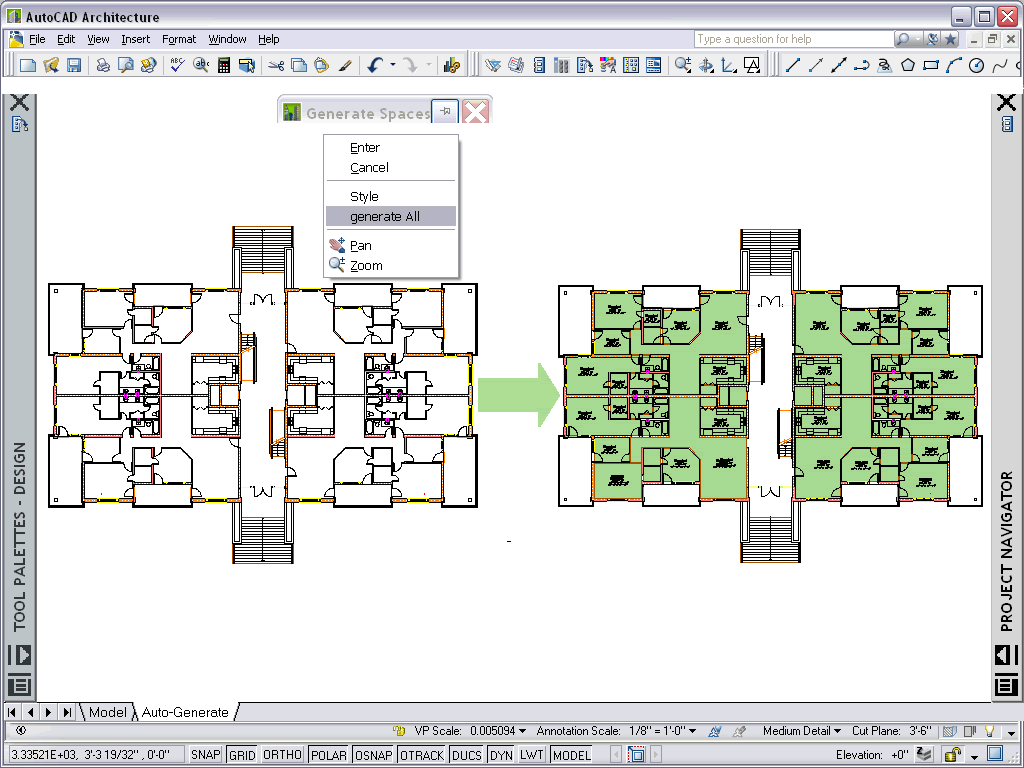
\includegraphics[width=.8\mycolumnwidth]{Introduccion_fundamentos/CAD.png}
\caption{\small Entorno de trabajo de una aplicación CAD.}
\label{Fig:CAD} 
\end{figure}

El CAD puede resultar suficiente para desarrollar algunas tareas propias de los SIG, en particular las relacionadas con el diseño cartográfico. No obstante, algunas circunstancias ponen de manifiesto las carencias de una herramienta CAD para sustituir completamente a un SIG, al tener requerimientos para los que esta no puede ofrecer una solución. Entre estos requerimientos cabe citar los siguientes:

\begin{itemize}
\item Análisis, modelización, y gestión avanzada de datos espaciales.
\item Trabajo con datos que cubren una gran superficie geográfica. Necesidad de utilizar diversos sistemas de proyección.
\item Edición de datos por usuarios de distinto perfil y de modo concurrente.
\end{itemize}

Por su parte, las siglas AM/FM(\emph{Automated Mapping/Facilities Management})\footnote{Cartografía Automatizada/Gestión de Servicios} de uso poco habitual en nuestro idioma, hacen referencia a aplicaciones diseñadas para la gestión de infraestructuras generalmente de carácter público, tales como redes de alcantarillado, conducciones de gas o vías de circulación, entre otras. 

Las aplicaciones empleadas para estas tareas tienen dos bloques básicos: un bloque gráfico de visualización y otro de gestión de datos. Este último almacena los atributos asociados a los elementos gráficos, que son principalmente de tipo lineal (tuberías, redes de alumbrado, etc.). Otro tipo de elementos, tales como elementos poligonales, son difíciles de manejar en estos sistemas, ya que su diseño obedece a las necesidades existentes en su ámbito de utilización, y estas se sitúan mayoritariamente alrededor de las infraestructuras lineales. Sin embargo, incluso con este tipo de elementos las capacidades de una aplicación AM/FM no igualan a las de un SIG, ya que no incorporan otro tipo de información como la relativa a la topología (que describiremos con detalle en el capítulo \ref{Tipos_datos}). Esto es así debido a que el subsistema de análisis, fundamental en un SIG, no tiene presencia en estas herramientas, y por tanto sus características no incluyen aquellos componentes que sean necesarios exclusivamente para procesos de tipo analítico.

Puede decirse, por tanto, que este tipo de aplicaciones representa un subconjunto de los SIG, pues sus funcionalidades principales son más reducidas que las de estos, y su ámbito de aplicación es menos generalista. En cierta medida, las aplicaciones AM/FM se asemejan también a las aplicaciones CAD, poniendo un énfasis especial en la componente gráfica, aunque con una mayor adaptación a la naturaleza geográfica de la información con la que se trabaja.

Al contrario sin embargo de lo que sucede con las aplicaciones CAD, en la actualidad las labores propias asociadas a los productos AM/FM se pueden llevar a cabo en un SIG genérico, o bien en una adaptación de este que tenga en consideración las características particulares del ámbito de trabajo. En este sentido, la gestión de servicios no es una aplicación más específica que otras a la hora de emplear un SIG, y este en la actualidad engloba de forma casi completa las funcionalidades de una herramienta AM/FM.

%
\section{Componentes de un SIG}

Como ya hemos visto, en su concepción actual los SIG son sistemas complejos que integran una serie de distintos elementos interrelacionados. El estudio de todos y cada uno de estos elementos es el fundamento para el estudio global de los Sistemas de Información Geográfica, y de ese modo se aborda a lo largo de este libro, mostrando las propias características de cada elemento y los conceptos necesarios para entender las relaciones entre ellos.

Una forma de entender el sistema SIG es como formado por una serie de subsistemas, cada uno de ellos encargado de una serie de funciones particulares. Es habitual citar tres subsistemas fundamentales:

\begin{itemize}
	\item Subsistema de \textbf{datos}. Se encarga de las operaciones de entrada y salida de datos, y la gestión de estos dentro del SIG. Permite a los otros subsistemas tener acceso a los datos y realizar sus funciones en base a ellos.
	\item Subsistema de \textbf{visualización y creación cartográfica}. Crea representaciones a partir de los datos (mapas, leyendas, etc.), permitiendo así la interacción con ellos. Entre otras, incorpora también las funcionalidades de edición.
	\item Subsistema de \textbf{análisis}. Contiene métodos y procesos para el análisis de los datos geográficos.
\end{itemize}

Para que un SIG pueda considerarse una herramienta útil y válida con carácter general, debe incorporar estos tres subsistemas en cierta medida\cite{ESRI2003ESRI}.

Otra forma distinta de ver el sistema SIG es atendiendo a los elementos básicos que lo componen. Cinco son los elementos principales que se contemplan tradicionalmente en este aspecto (Figura \ref{Fig:Elementos_SIG}):

\begin{itemize}
 \item \textbf{Datos}. Los datos son la materia prima necesaria para el trabajo en un SIG, y los que contienen la información geográfica vital para la propia existencia de los SIG.
\item \textbf{Métodos}. Un conjunto de formulaciones y metodologías a aplicar sobre los datos.
\item \textbf{Software}. Es necesaria una aplicación informática que pueda trabajar con los datos e implemente los métodos anteriores.
\item \textbf{Hardware}. El equipo necesario para ejecutar el software.
\item \textbf{Personas}. Las personas son las encargadas de diseñar y utilizar el software, siendo el motor del sistema SIG.
\end{itemize}

\begin{figure}[h]   
\centering
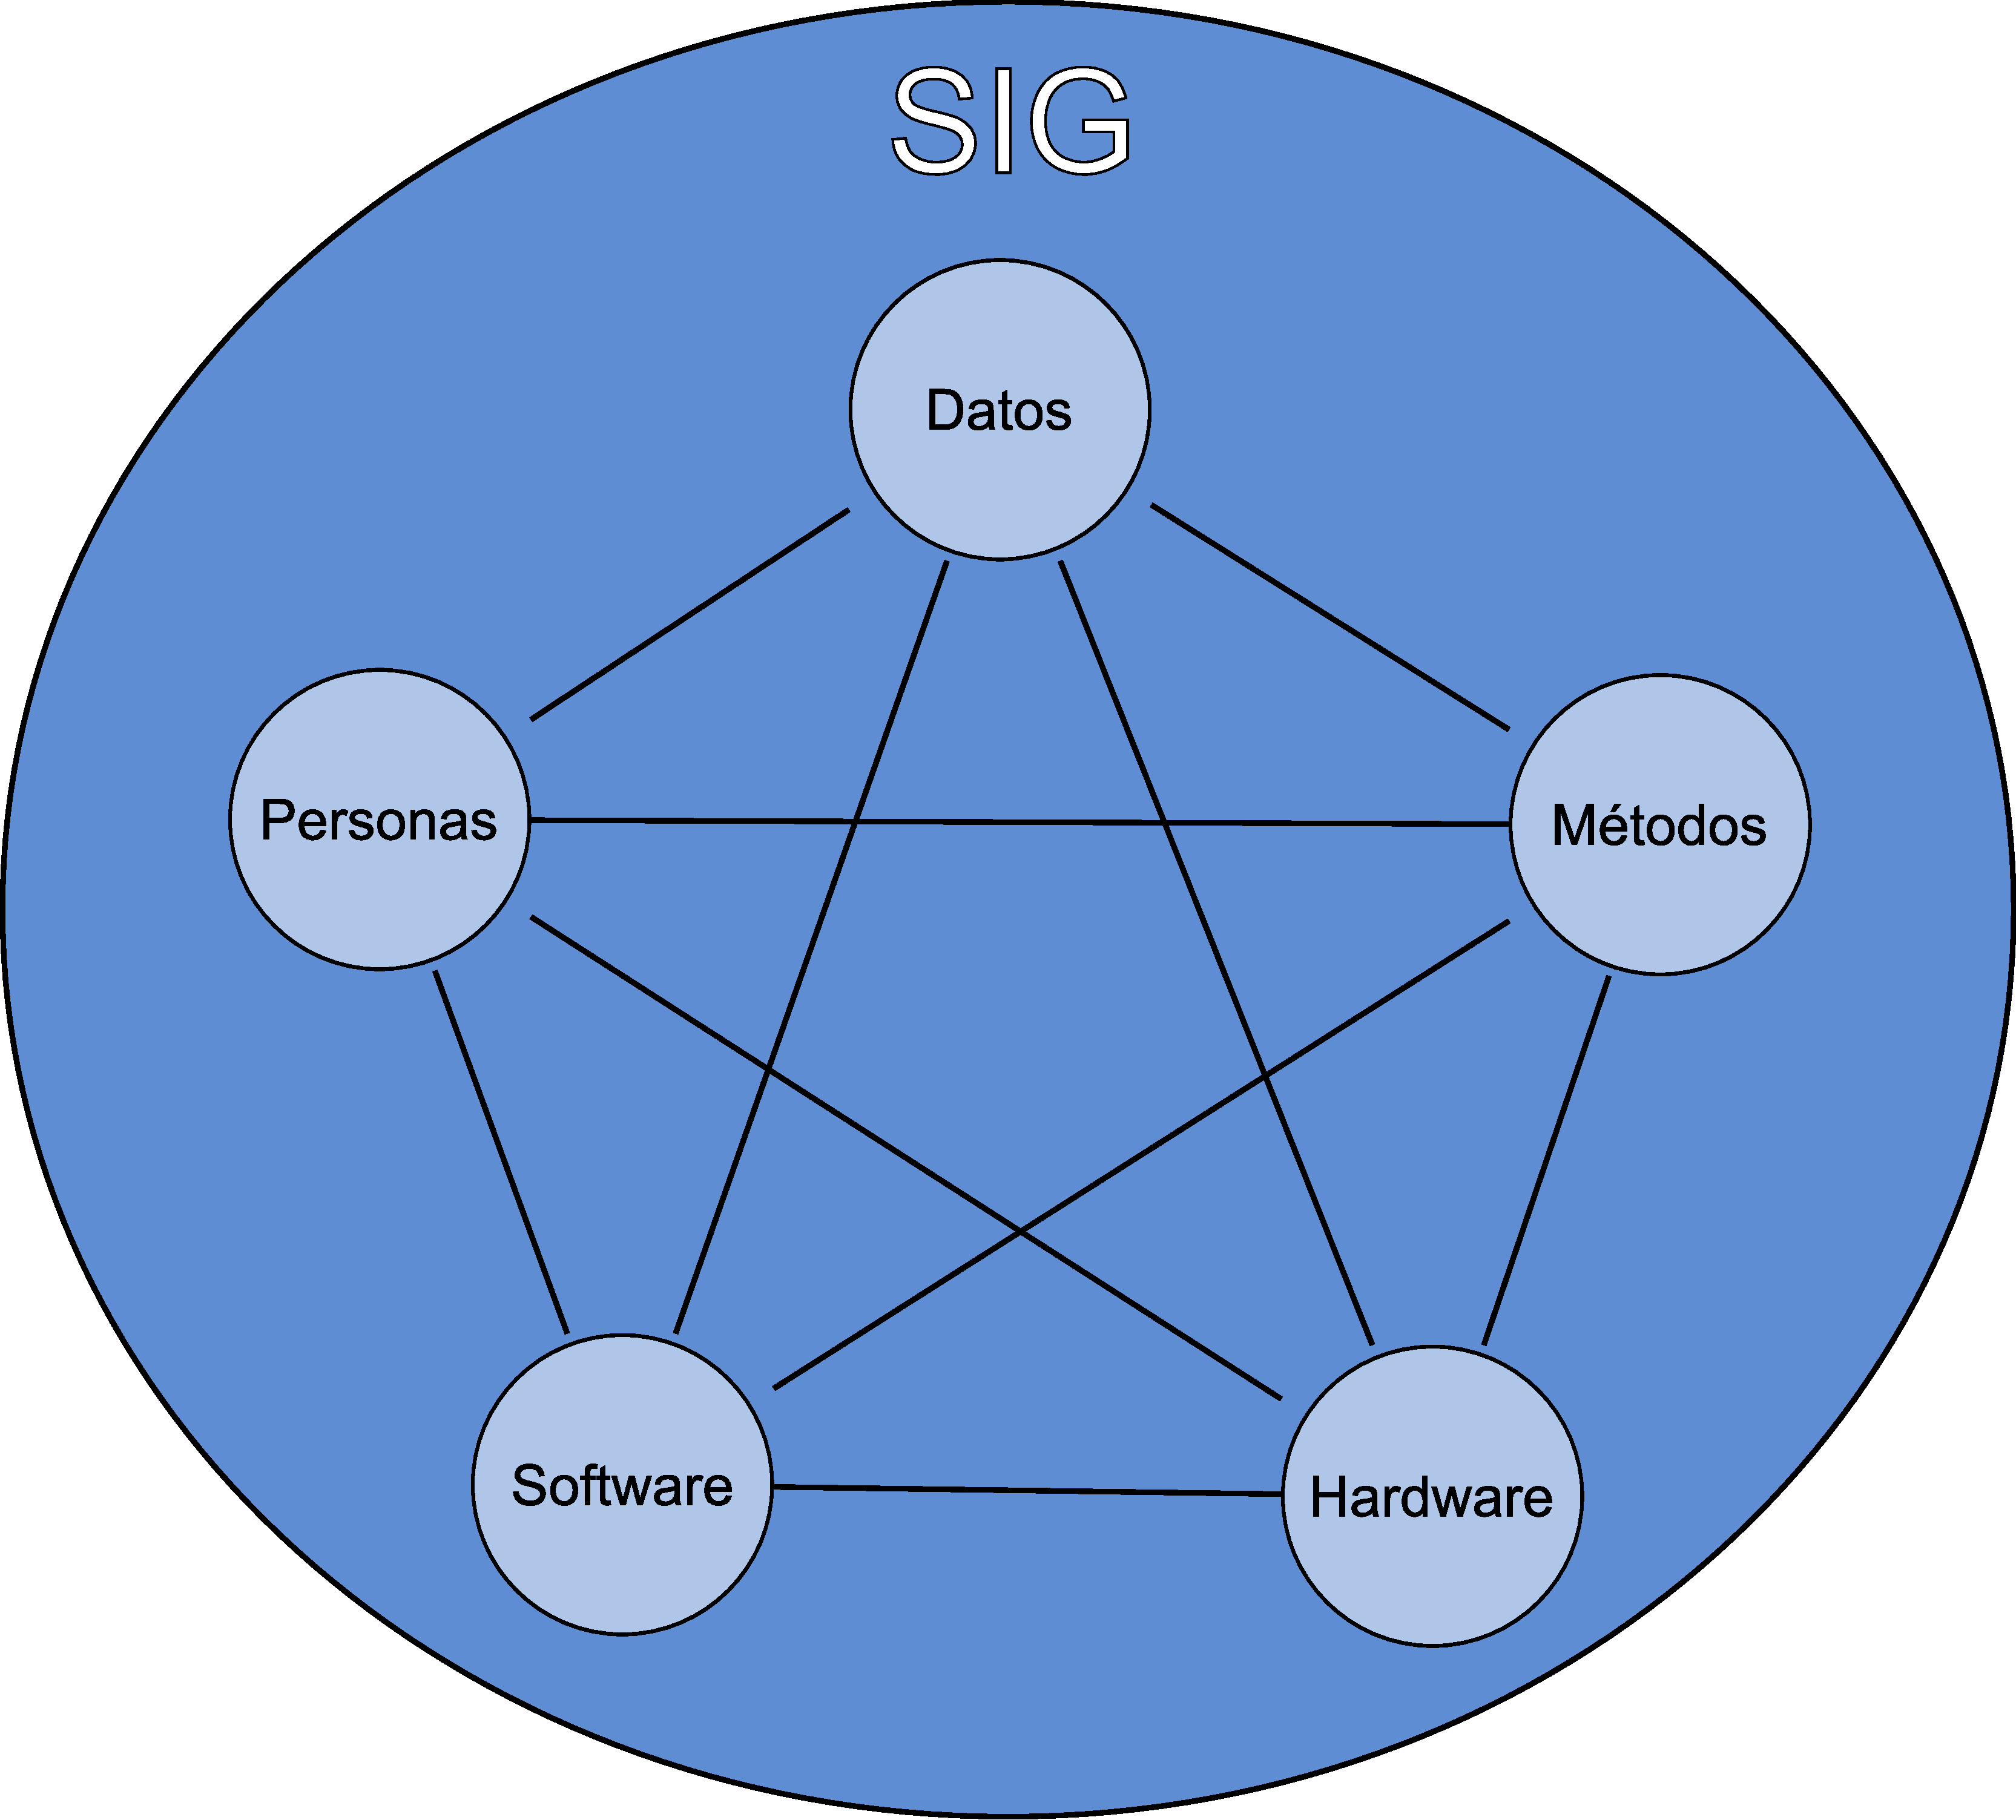
\includegraphics[width=.55\mycolumnwidth]{Introduccion_fundamentos/Elementos_SIG.pdf}
\caption{\small Elementos que forman el sistema SIG}
\label{Fig:Elementos_SIG} 
\end{figure}

Para el enfoque de esta obra, cada uno de los elementos anteriores tiene unas características propias que deben estudiarse. No obstante, el hardware no es un elemento especialmente particular en el caso de un SIG, y las aplicaciones SIG que encontramos actualmente en el mercado en todas sus variedades (que son las que el lector de este libro va a utilizar habitualmente) se ejecutan en su mayoría sobre ordenadores personales sin requerimientos altamente específicos. Más aún, la expansión de las tecnologías SIG ha alcanzado hoy en día otros ámbitos como las plataformas móviles, haciendo de estas unas tecnologías poco específicas en lo que a \emph{hardware} se refiere. Por esta razón, no es necesario tratar en detalle esta pieza del sistema SIG, siendo más adecuado tratar el resto de elementos, más característicos e importantes para el aprendizaje de los conceptos SIG y la descripción de estos.

Por su parte, las personas tienen importancia tanto de forma individual como en su conjunto, siendo diferentes las necesidades que plantean como usuarios y beneficiarios de un SIG. En la sociedad actual, las tecnologías y planteamientos colaborativos han calado hondo en el ámbito SIG, y la información geográfica es, por su propia naturaleza, propensa a ser compartida y utilizada por diferentes personas con fines muy distintos. Es por ello que el aspecto de mayor relevancia respecto a las personas como partes del sistema SIG es el de sus relaciones y su organización, siendo además en este campo donde se han producido en mayor medida los últimos avances, y donde ha tenido lugar un cambio más profundo, no ya solo dentro de los SIG, sino también en otras tecnologías de similar índole.

Puede entenderse esto como un nuevo subsistema: el subsistema \emph{de gestión}, que es responsable de gestionar la interacción de los restantes y definir y controlar el marco en que esta tiene lugar.

Las personas a su vez dan forma a los distintos ámbitos de trabajo, definiendo estos en función de sus necesidades. Puede tratarse el conjunto de campos de especialización como un nuevo elemento del sistema SIG, en lugar de incorporarlo dentro de otro. 

Algunos autores proponen modificar el esquema clásico de cinco elementos para reflejar más correctamente la nueva realidad de los SIG. Por ejemplo, \cite{webGISEvolve} propone un esquema como el mostrado en la figura \ref{Fig:Elementos_SIG2}.

\begin{figure}[h]   
\centering
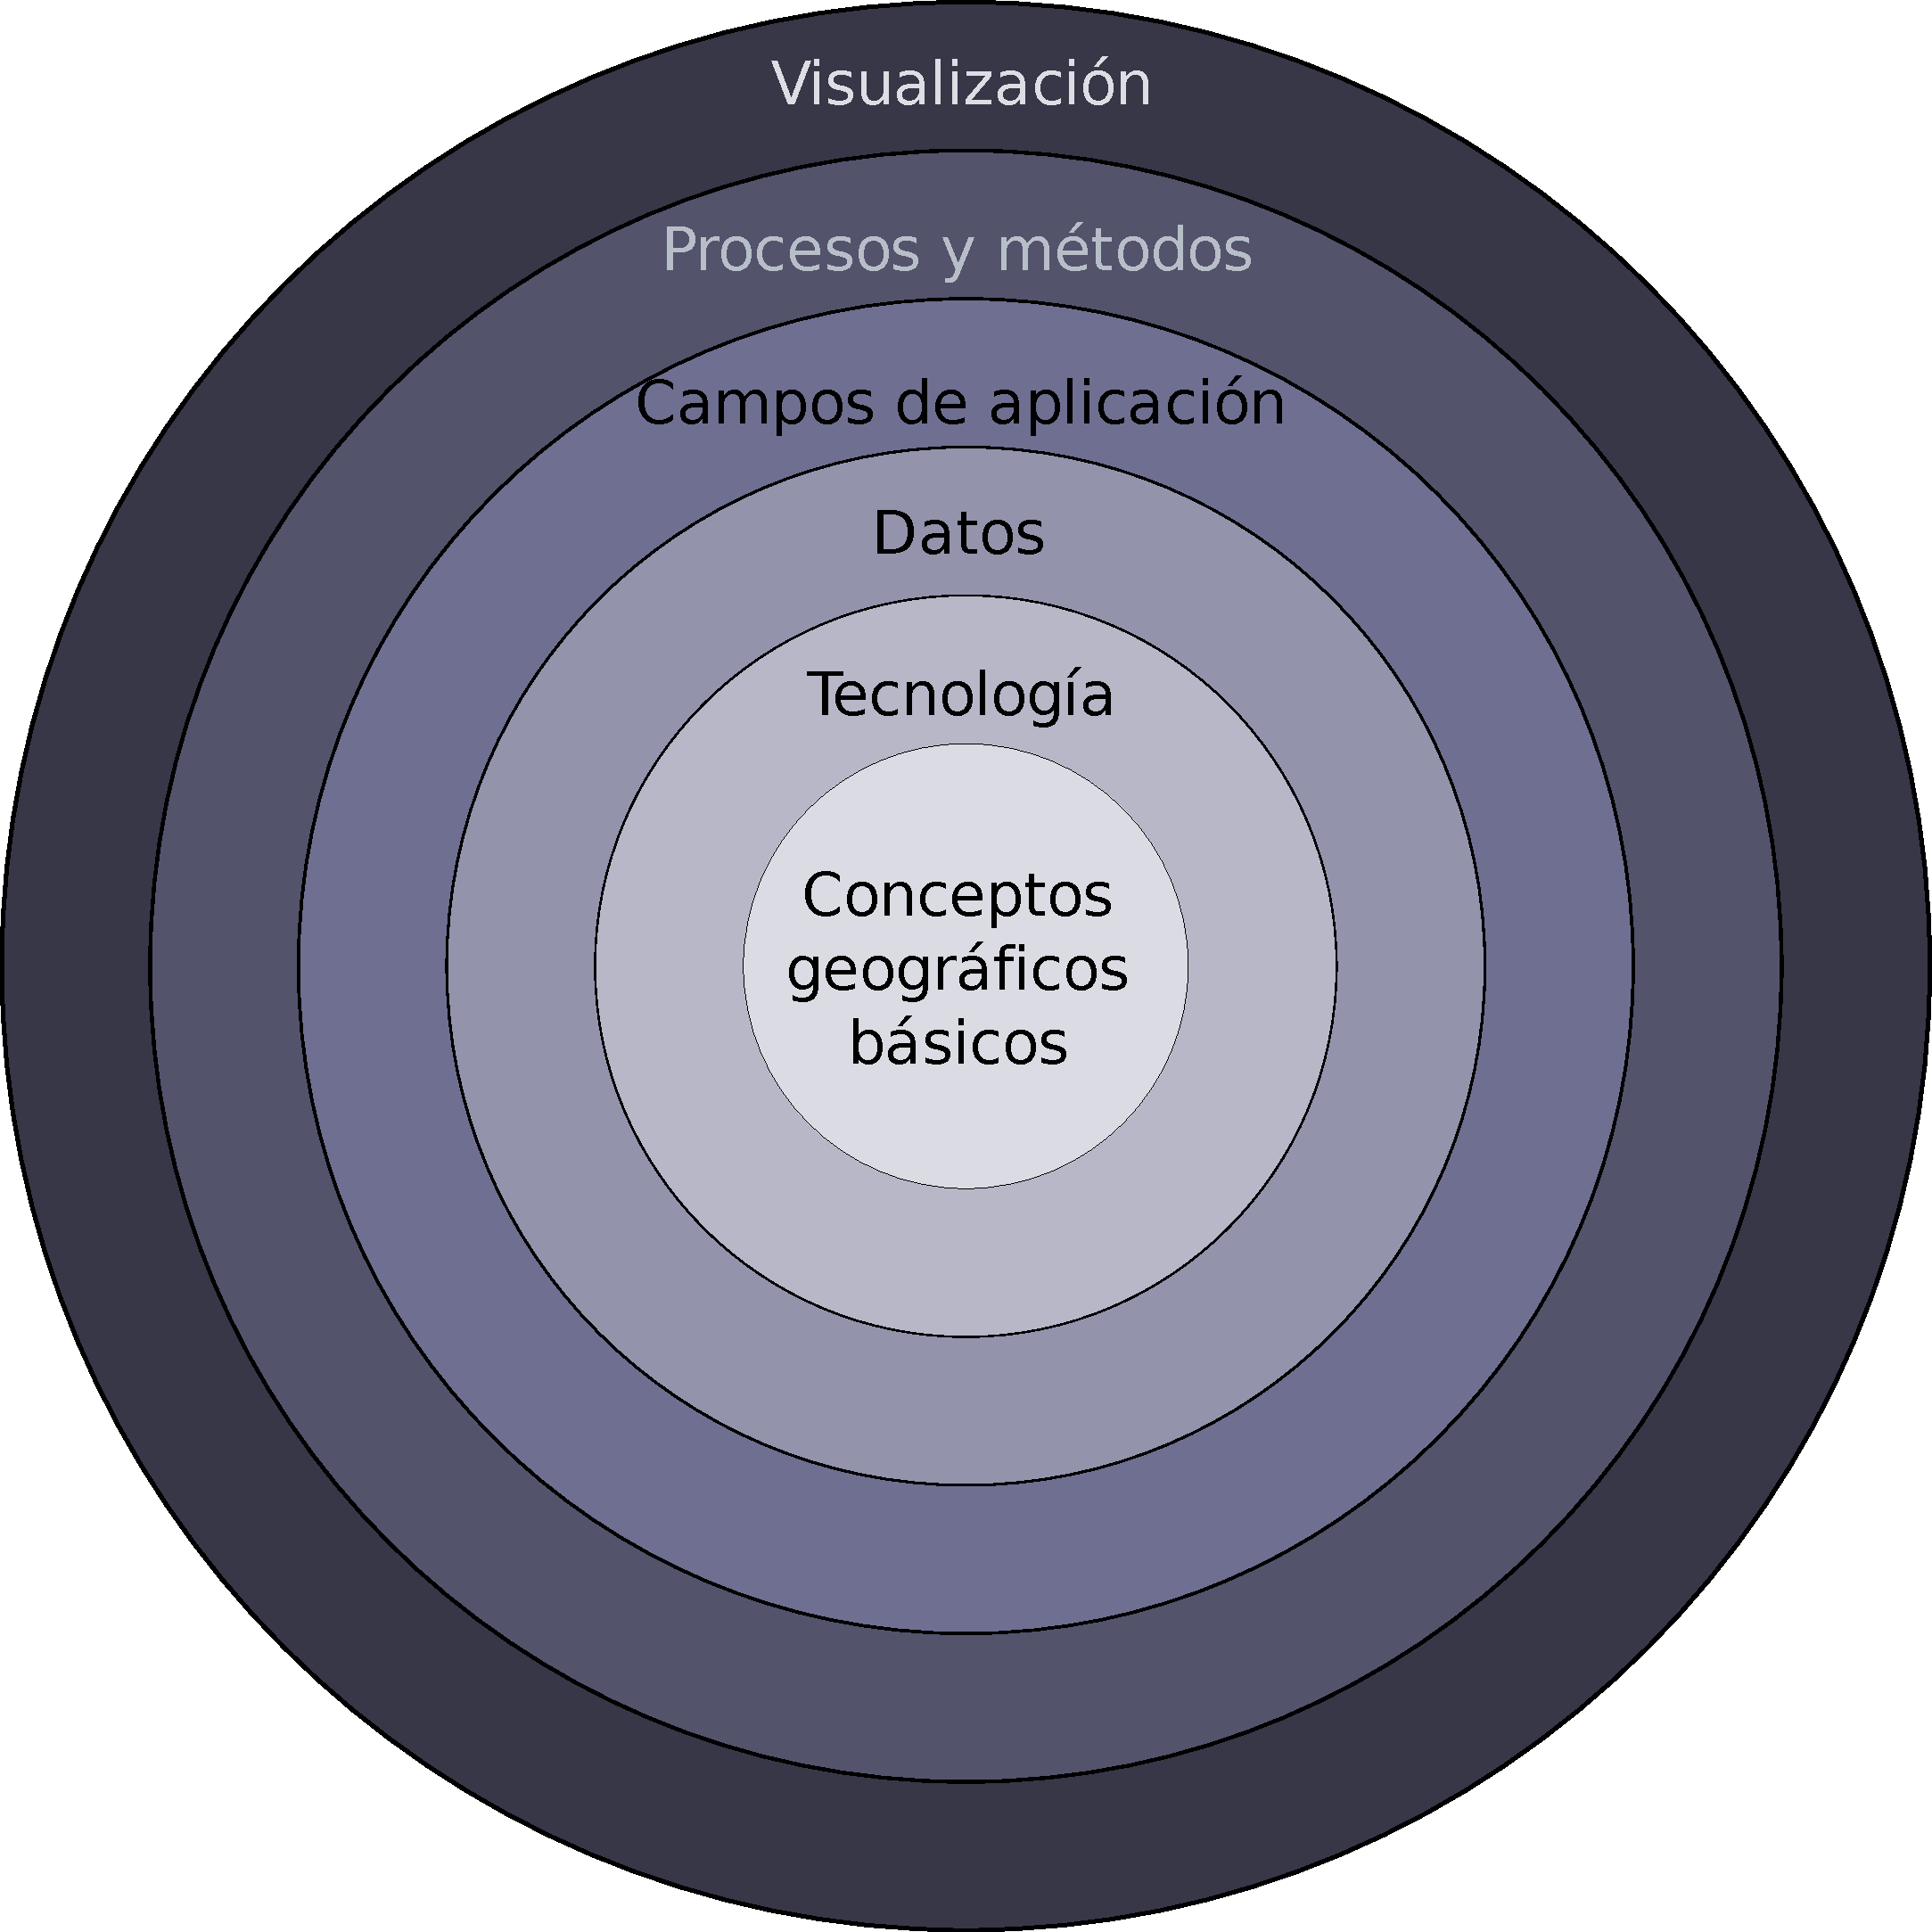
\includegraphics[width=.55\mycolumnwidth]{Introduccion_fundamentos/Elementos_SIG2.pdf}
\caption{\small Una división distinta del sistema SIG (según \cite{webGISEvolve})}
\label{Fig:Elementos_SIG2} 
\end{figure}

La incorporación de la visualización es una diferencia notable con respecto al esquema clásico. En realidad, y si volvemos a ese enfoque basado en subsistemas, el subsistema de visualización resulta de enorme importancia en un SIG, siendo pese a ello habitual que no sea tratado con la suficiente profundidad en textos dedicados a los SIG desde un punto de vista genérico. Precisamente por no ser considerado un elemento independiente, no se le concede la necesaria atención como parte que debe estudiarse al tratar la disciplina de los SIG.

Esto contrasta con el hecho de que, a pesar de que las capacidades de los SIG son mucho más amplias que las relacionadas con la visualización, muchos usuarios usan estas por encima de las restantes, desconociendo incluso en muchos casos gran parte de las otras capacidades que un SIG puede brindarles. Correcto o no, desde el punto de vista del usuario medio, las capacidades de visualización están en primera línea del conjunto de funcionalidades de un SIG.

Abordar el estudio de un SIG acudiendo al esquema clásico de cinco elementos deja de lado la visualización, en cuanto que la engloba como una funcionalidad derivada de dichos elementos en su conjunto pese a que esta tiene unas características peculiares en el entorno de un SIG y una vital importancia en la concepción actual de este. Es decir, el esquema de partes de un SIG no resulta el más adecuado para estructurar el estudio de los SIG, al menos en lo que respecta a la visualización como parte fundamental de estos.

El objetivo de este libro es tratar con suficiente detalle y rigor todos los aspectos fundamentales de un SIG, incluyendo, por supuesto, la visualización de datos geográficos. Para ello, es conveniente tratar también esta desde un punto de vista teórico, detallando los fundamentos en los que se basa y que, pese a ser de vital importancia para el uso de un SIG, son ignorados frecuentemente. 

Con todo lo anterior, resulta más conveniente para su estudio práctico adoptar una evolución del esquema clásico de cinco elementos, y establecer unos nuevos componentes, cada uno de los cuales actúa como un pilar conceptual sobre el que ha de sustentarse es estudio de la disciplina de los SIG. Estos componentes son cinco:

\begin{itemize}
 \item Datos.
\item Análisis. Métodos y procesos enfocados al análisis de los datos.
\item Visualización. Métodos y fundamentos relacionados con la representación de los datos. 
\item Tecnología. \emph{Software} y \emph{hardware} SIG
\item Factor organizativo. Engloba los elementos relativos a la coordinación entre personas, datos y tecnología, o la comunicación entre ellos, entre otros aspectos.
\end{itemize}

A modo de introducción, se describen a continuación algunas ideas básicas de cada uno de estos componentes. Salvo el factor organizativo, cuyos elementos se explicarán a lo largo de toda esta obra, el resto de componentes se detallarán individualmente, cada uno de ellos en una parte correspondiente del libro.


\subsection{Datos}

Los datos son necesarios para hacer que el resto de componentes de un SIG cobre sentido y puedan ejercer su papel en el sistema. La información geográfica, la verdadera razón de ser los SIG, reside en los datos, y es por ello que el conocimiento exhaustivo de los datos y su naturaleza resulta obligado para una buena comprensión los propios SIG.

Son muchas las facetas de los datos que deben estudiarse, y todas ellas con una gran importancia. Por un lado, es necesario conocer las características fundamentales del dato geográfico que utilizamos en un SIG, es decir, su forma y sus propiedades. De ellas dependen, por ejemplo, los procesos que podremos o no realizar con los datos, y en general todo cuanto podemos esperar de ellos.

Prescindiendo del hecho de que se trata de un dato geográfico, es relevante conocer cómo los datos se gestionan y almacenan en un entorno digital, aspectos de corte puramente informático que desarrolla la disciplina de la gestión de bases de datos. Cuando las ideas fundamentales al respecto se aplican al caso particular de los datos geográficos, surgen conceptos que resultan básicos para un buen uso de un SIG, y que además van siendo cada vez más relevantes a medida que los volúmenes de datos de que se dispone van aumentando. 

Al igual que aumenta el volumen de datos, lo hacen los orígenes de estos y las formas en que la información geográfica puede recogerse. Un aspecto clave para una utilización correcta de un SIG es saber integrar datos de distinta procedencia, para lo cual es vital entender cómo esta afecta a las propias características de dichos datos.

Otros elementos tales como la calidad de los datos, la cual cobra cada día más importancia, serán tratados igualmente junto a los anteriores en una parte específicamente dedicada a los datos, probablemente una de las más importantes dentro de este libro.

\subsection{Análisis}

El análisis es una las funcionalidades básicas de los SIG, y una de las razones fundamentales que llevaron al desarrollo de estos. Un ordenador es una herramienta con enorme capacidad de cálculo, y esta puede aplicarse a los datos espaciales para obtener resultados de muy diversa índole.

En mayor o menor medida, un SIG siempre incorpora una serie de formulaciones que permiten la obtención de resultados y el análisis de los datos espaciales. Estas formulaciones representan procesos que pueden ser sumamente sencillos o enormemente complejos, y que pueden resultar de aplicación en uno u otro campo, o incluso con carácter general. Su origen puede ser muy variado, y no derivan  necesariamente del ámbito puro de la geografía, sino que pueden ir desde simples consultas o mediciones a elaborados modelos que empleen datos de variables muy numerosas y arrojen resultados complejos. La estadística, entre otras ciencias, puede aportar al ámbito SIG muchas de sus ideas, y estas, adaptadas al marco de la información georreferenciada, constituir en el SIG un nuevo conjunto de procesos de análisis.

Las ventajas de la incorporación de todos estos procesos en una única herramienta, el SIG, van desde la automatización de tareas a la aparición de nuevos procesos que, aprovechando la gran capacidad de cómputo de la plataforma en la que se ejecuta el SIG, producen resultados que no podrían ser obtenidos de otro modo. Bien sea por la complejidad propia de los procesos o por el nivel de precisión al que se trabaja, existen muchos procesos que mediante el uso de cartografía clásica y sin el apoyo de medios informatizados no pueden realizarse. El SIG abre un campo de actuación en el que la práctica totalidad de ideas y formulaciones de análisis pueden plasmarse y aplicarse con carácter práctico.


\subsection{Visualización}

Cualquier tipo de información puede ser representada de forma gráfica, lo cual habitualmente facilita la interpretación de dicha información o parte de esta. Gran parte de las características de la información (por ejemplo, la presencia de patrones sistemáticos), son más fáciles de estudiar cuando se apoyan sobre algún elemento visual, pues este añade un nuevo punto de vista.

En el caso particular de la información geográfica, la visualización no solo es una forma más de trabajar con esa información, sino que resulta la forma principal, no ya por ser la que en general hace más fácil e intuitivo el tratamiento de esa información, sino porque es aquella a la que estamos más acostumbrados. La información geográfica tiene una inherente naturaleza visual, ya que el espacio en sí es entendido de forma gráfica por el ser humano. Junto a esto, no debemos olvidar que la información geográfica se ha almacenado de forma tradicional de modo también visual, a través de mapas. Un mapa es en sí una representación visual de la información geográfica.

Al contrario que un mapa, que de por sí es de naturaleza gráfica, en un SIG trabajamos con datos de tipo puramente numérico, ya que es así como el ordenador puede manejarlos, y la información geográfica debe almacenarse de este modo, como veremos con detalle en el capítulo \ref{Tipos_datos}. Para poder presentar una utilidad similar a la de un mapa en lo que a la presentación de la información respecta, un SIG debe incluir capacidades que generen representaciones visuales a partir de esos datos numéricos, aprovechando en la medida de lo posible las propias capacidades del medio informático en que se trabaja para hacer estas representaciones más potentes como transmisoras de información. 

Es deseable igualmente que el SIG sea capaz de generar cartografía clásica, y que incorpore métodos para el diseño cartográfico y la creación de mapas impresos, pues estos no pierden su vigencia pese a la existencia de los SIG.

La visualización de la información geográfica se rige por los mismos conceptos y principios que se emplean para la confección de cartografía impresa, y estos deben ser conocidos por el usuario de SIG, ya que una de las tareas de este es el diseño cartográfico y las preparación de los elementos de visualización para poder realizar su trabajo sobre las representaciones creadas. A los conceptos tradicionales hay que sumar algunas ideas nuevas, ya que un SIG es capaz de generar representaciones más avanzadas (por ejemplo, representaciones tridimensionales). A esto hay que sumar la presencia de un elemento característico y de gran importancia como es la elevada interactividad que toda representación gráfica lleva asociada dentro de un SIG, y que constituye una gran diferencia frente al carácter estático de la cartografía clásica.

Por todo ello, la visualización debe considerarse como un componente fundamental del sistema SIG en su concepción actual, y particularmente uno con especial interés desde el punto de vista del usuario directo de tecnologías SIG.

\subsection{Tecnología}

Incluimos en este elemento tanto el \emph{hardware} sobre el que se ejecutan las aplicaciones SIG, como dichas aplicaciones, es decir el \emph{software} SIG. Ambos forman un binomio tecnológico en el que encontramos diversas alternativas, y que se enriquece diariamente con la rápida evolución del mercado tecnológico.

En lo que a \emph{hardware} respecta, es el elemento físico del sistema SIG, y conforma la plataforma sobre la que tiene lugar el trabajo con un SIG. La utilización de un SIG hoy en día se puede llevar a cabo en ordenadores personales o estaciones de trabajo, y ya sea de forma individual o en una arquitectura cliente--servidor más compleja. Estas últimas han cobrado importancia muy rápidamente en los últimos tiempos, especialmente en lo que al acceso a datos se refiere. Veremos más adelante como esto también ha tenido influencia en otros componentes del sistema SIG, principalmente en el factor organizativo.

Además de la propia plataforma, el \emph{hardware} incluye una serie de periféricos para tareas más concretas. De uso habitual en el trabajo con SIG son los periféricos para entrada de datos geográficos y la creación de cartografía. Las tabletas digitalizadoras son la forma más habitual dentro del primer grupo (las veremos con más detalle en el apartado \ref{heads-down}), mientras que \emph{plotters}\index{Plotter} e impresoras son empleados para la creación cartográfica, requiriéndose generalmente un mayor formato que para otros usos.

Más recientemente, la aparición de Sistemas de Navegación Global\index{Sistemas de Navegación Global} como el GPS\index{GPS} (que pueden a su vez considerarse como otro tipo de periféricos) ha creado una parcela tecnológica con gran relación con los SIG, convirtiendo a estos en herramientas ideales para la gestión de los datos de dichos sistemas. Incluso, la combinación de SIG y GPS sobre un único elemento de hardware ha dado lugar a herramientas como los navegadores GPS, que han supuesto un hito no solo desde el punto de vista técnico, sino también desde un enfoque social, pues acercan las tecnologías SIG a usuarios no expertos.

Por su parte, el \emph{software} es el encargado de operar y manipular los datos. El software SIG también ha sufrido una gran evolución, y bajo el paraguas de esa denominación encontramos desde las aplicaciones clásicas que permiten visualizar, gestionar y analizar los datos geográficos, hasta herramientas más especializadas que se centran en alguno de estos campos, o bien componentes que pueden incluso pasar a formar parte de otras aplicaciones fuera del ámbito SIG, pero que puntualmente requieren algunas de sus funcionalidades, especialmente las relacionadas con la visualización de cartografía digital.

\subsection{Factor organizativo}

El sistema SIG requiere una organización y una correcta coordinación entre sus distintos elementos. El factor organizativo ha ido progresivamente ganando importancia dentro del entorno SIG, a medida que la evolución de estos ha ido produciendo un sistema más complejo y un mayor número de intrarelaciones e interrelaciones entre los distintos componentes que lo forman.

Especialmente importante es la relación entre las personas que forman parte del sistema SIG, así como la relación de todos los elementos con los datos, sobre los cuales actúan de un modo u otro. Ello ha propiciado la aparición de, entre otros, elementos que pretenden estandarizar los datos y gestionar estos adecuadamente.

Cuando los SIG se encontraban en sus etapas de desarrollo iniciales y eran meras herramientas para visualizar datos y realizar análisis sobre ellos, cada usuario tenia sus propios datos con los cuales trabajaba de forma independiente del resto de usuarios, incluso si estos llevaban a cabo su trabajo sobre una misma área geográfica y estudiando las mismas variables. Hoy en día, la información no se concibe como un elemento privado de cada usuario, sino como un activo que ha de gestionarse, y del que deriva toda una disciplina completa.La aplicación de esta disciplina es la base de algunos de los avances más importantes en la actualidad, teniendo implicaciones no ya solo técnicas sino también sociales en el ámbito de los SIG.

Asimismo, las necesidad de gestión de los datos y la propia complejidad de un SIG, provocan ambas que no exista un perfil único de persona involucrada en el sistema SIG, sino varias en función de la actividad que desarrollen. Al usuario clásico de SIG se unen las personas responsables de gestionar las bases de datos, las encargadas de diseñar la arquitectura de un SIG cuando este se establece para un uso conjunto por parte de toda una organización o grupo de mayor entidad. Dentro de las personas que participan en un SIG, el usuario directo es el eslabón último de una cadena que incluye igualmente a otros profesionales con roles bien distintos.

Incluso atendiendo únicamente a los usuarios, también entre estos existen diferentes perfiles, y las comunidades de usuarios no expertos juegan en la actualidad un importante papel en el mundo del SIG. Esta situación, a su vez, requiere elementos organizativos importantes. Con la popularización y bajo coste de las unidades GPS y la aparición de la denominada Web 2.0, el SIG ha llegado a usuarios no especializados, los cuales utilizan estas herramientas para la creación y uso de su propia cartografía, dentro de lo que se conoce como VGI (\emph{Volunteered Geographic Information}\footnote{Información geográfica creada voluntariamente}) \cite{goodchildVGI}. El término \emph{Neogeografía}, de reciente creación, hace referencia a este uso de los SIG y otras herramientas asociadas por parte de grupos de usuarios no especializados.

En definitiva, resulta necesario gestionar correctamente la complejidad del sistema SIG, y esta gestión se ha convertido ya en un elemento fundamental dentro del entorno SIG actual.

\section{Resumen}

En este capítulo hemos presentado los SIG como herramienta para el manejo general de información geográfica, fundamental para trabajar hoy en día con todo tipo de información georreferenciada. Un SIG es un sistema compuesto por cinco piezas fundamentales: datos, tecnología, análisis, visualización y factor organizativo. Cada una de ellas cumple un papel determinado dentro del sistema SIG, el cual se caracteriza fundamentalmente por su naturaleza integradora. 

Existen otras herramientas y tecnologías que pueden en principio asemejarse a los SIG, pero que realmente no comparten con estos su capacidad de integrar bajo un marco común una serie completa de elementos y disciplinas, siendo esta la verdadera propiedad que define a los SIG.

Todo el conjunto de conocimientos sobre los cuales se asientan los SIG conforman la denominada Ciencia de la Información Geográfica. Bajo esta denominación se recogen todos los temas a tratar en esta obra.

\pagestyle{empty}
